\chapter{\label{c:gw-detection}Gravitational waves}

\note{The effect of GWs on our detectors is proportional to their amplitude which means the signal rises in proportion as the distance falls. (It is not like detecting photons, which is a measurement of the signal power, when we get the familiar 1/r2 law.)}

\section{Event GW150914}
\checkme{One billion years ago}, a pair of black holes, one with 36 solar masses and another with 29 solar masses, merged into a single black hole with 62 solar masses. The missing energy equivalent to 3 solar masses was radiated away in the form of gravitational waves.

At 09:50:45 \gls{UTC} on \nth{14} September 2015, gravitational waves from the black hole passed through the LIGO Livingston detector, perturbing the mirrors by \checkme{\SI{e-18}{\meter}} and creating a signal large enough for the electronics controlling the interferometer to detect the ripple in space time more than \checkme{23} times above the noise. Seven milliseconds later, the same wavefront passed the LIGO Hanford detector and moved the mirrors in the opposite direction. At that moment, for the first time in human history, a gravitational wave had been detected.

From the gravitational waveform witnessed at the LIGO sites it was possible to determine the type and parameters of the waves' source. \emph{GW150914}'s waveform can be observed in Figure\,\note{ADD FIGURE}. This waveform, consistent with a binary black hole merger, swept up in frequency (the \emph{inspiral}) before combining (the \emph{merger}) and creating an audible ``chirp''. The signal was only above each detector's noise level from a frequency of around \checkme{x}. Not only did LIGO make the first observation of a gravitational wave, it also made the first detection of a binary black hole system. The window into the universe opening up due to the LIGO\textemdash and the worldwide network of gravitational wave detectors in operation and under assembly, GEO-600, Virgo and KAGRA\textemdash represents a new opportunity to study the universe in a completely different way. Some secrets have already been learned, but there are surely many more to be uncovered. Although this is just the beginning of gravitational astronomy, work is already under way to produce bigger and better gravitational wave detectors both on the Earth and in Space.

\subsection{Scientific outcomes from the first LIGO science run}
\note{GWs exist, first direct observation of BH, BBH merger, high mass, relativity tested in strong gravity, etc.}

\subsection{Possible future discoveries}
\note{CBCs, stochastic background, etc.}

\section{General relativity and gravitational waves}
A consequence of Einstein's theory of general relativity, gravitational waves are produced by changes in the quadrupole moment of a distribution of mass. Changes in the lower order monopole and dipole terms are forbidden due to energy and momentum conservation, meaning that the effect a gravitational wave has on spacetime is to stretch it in one direction while contracting it in another. This strain can be expressed as a linear combination of ``plus'' and ``cross'' polarisation terms, shown for an initially circular ring of test particles as a function of phase angle in Figure\,\ref{fig:gravitational-wave-polarisation}.

\begin{figure}
  \centering
  \includegraphics[width=\columnwidth]{graphics/generated/from-svg/10-gravitational-wave-polarisation.pdf}
  \caption[Plus and cross polarisations of a propagating gravitational wave]{\label{fig:gravitational-wave-polarisation}Plus and cross polarisations of a propagating gravitational wave. As the wave travels, it stretches spacetime in one direction while contracting it in the other in an elliptic behaviour. A gravitational wave's propagation can be described as a linear combination of the two polarisations.}
\end{figure}

\subsection{Sources}
Gravitational waves from Earth-bound mass distributions, including the Earth itself, are not even remotely detectable. The strain in spacetime produced by such objects is so weak that there is no hope for us to make such a detection with any known technology. A good estimate for the strain produced by a pair of rotating objects is given in \cite{Sathyaprakash2009} as\footnote{Note that the equation in question, (9) in \cite{Sathyaprakash2009}, has been converted here into SI units.}:
\begin{equation}
  \label{eq:happrox}
  h \lesssim \frac{2 G \left( M v^{2} \right)_{\text{nonspherical}}}{c^4 r},
\end{equation}
where $G$ is the gravitational constant, $\left( M v^{2} \right)_{\text{nonspherical}}$ is the kinetic energy associated with the non-spherical parts of the source, $c$ is the speed of light and $r$ is the distance to the source. To get an idea of what the spacetime strain would be for man-made sources, we can consider as in \cite{Sathyaprakash2009} the case of two cars of mass $M = \SI{e3}{\kilo\gram}$ attached to opposite ends of a rod of length $d = \SI{10}{\meter}$, spinning about its centre in a centrifuge at a frequency of $f = \SI{10}{\hertz}$. The tangential velocity of the cars will be around $2 \pi f d \approx \SI{600}{\meter\per\second}$. Placing the detector one wavelength away, and using Equation\,\ref{eq:happrox}, the strain turns out to be around $\SI{4e-43}{}$. To be able to detect such a strain, Advanced LIGO would require an improvement in sensitivity of \SI{20}{} orders of magnitude, which is clearly ludicrous.

A pair of solar-mass objects orbiting each other at \SI{100}{\hertz} within \SI{50}{\mega\lightyear} produces a strain of only one part in \SI{e21}{}, which is a strain only now detectable after decades of detector development, and a feat thought almost impossible by scientists of the early \nth{20} Century. It is only the waves produced by the most massive objects in the universe which we have any chance of detecting with the state of the art: black holes, neutron stars and supernovae, amongst others. Even then, gravitational radiation is only produced by the presence of a changing quadrupole moment, and so only a subset of sources that happen to be in coalescence or contain surface asymmetries produce waves we have the ability to detect.

\subsubsection{Compact binary coalescence}
As detected by LIGO in 2016...

\note{Show a picture of the waveform, with annotations - it might be available from https://wiki.ligo.org/viewauth/EPO/DiscoveryTalks.}

\subsubsection{Core collapse}
\note{Look up numbers from that rates paper.}

\subsubsection{Continuous wave}
\note{Pulsars}

\subsubsection{Stochastic background}
CMB...

\section{Multi-messenger astronomy}
From Equation\,\ref{eq:happrox} we can see that gravitational waves propagate with a $\frac{1}{r}$ law, in that the amplitude of a wave decays as the linear inverse of distance $r$. Contrast that to electromagnetic radiation, with which virtually all astronomy has thus far been conducted, where the $\frac{1}{r^2}$ law limits precision. Although gravitational waves are incredibly weak, they offer a glimpse into the structure and workings of the universe far out into the universe. Combined observations in the electromagnetic and gravitational wave spectrum allow researchers to learn even more about the universe, and this combined use of information carriers is called \emph{multi-messenger} astronomy. On one side, so-called \emph{electromagnetic follow-up} can be carried out after a gravitational wave detection to learn more about the source, given a sky localisation heavily limited by the presence of only two advanced detectors currently online. Another aspect of this astronomy is the ability for visual observations of events such as supernovae to focus analysis efforts of the vast quantities of detector data produced by the gravitational wave observatories. The eventual inclusion of new detectors in a worldwide network of gravitational wave observatories will herald an unprecedented ability to study our universe.

\section{Development of the gravitational wave detector}
The field of experimental gravitational wave detection began with Joseph Weber's studies in the 1960s \cite{Weber1960}. His \emph{Weber bar} was developed to act as a strain meter, with piezoelectric sensors placed on the surface of an aluminium cylinder to convert changes in length into electrical signals. Whilst the expected change in length of such a cylinder from gravitational radiation would in most cases be tiny---\checkme{of the order \SI{1e-22}{\meter} for a particularly loud source}---the resonant frequency of the cylinder, typically in the kilohertz range, acts to enhance the amplitude of the length change. The sensitivity of such a bar as a function of frequency is determined in part by its quality factor (Q), with a necessary trade-off being made between peak sensitivity (high Q) and detection bandwidth (low Q). As sources of gravitational radiation are almost universally weak, the only reasonable hope of making such a detection is to choose a high Q material and hope for a favourable signal frequency.

\begin{figure}
  \centering
  \includegraphics[width=0.5\textwidth]{graphics/generated/from-svg/10-michelson.pdf}
  \caption[]{Blah blah blah}
\end{figure}

The original resonant bar detectors were evolved over time to become cryogenic, to decrease the effect of thermal noise; and spherical, to maximise the test mass's Q. Despite such improvements the peak sensitivity of state-of-the-art resonant bar detectors was surpassed by interferometric gravitational wave detectors in 2003 \cite{Pitkin2011} after it was shown that second generation detectors would offer superior sensitivity across a much wider bandwidth\footnote{Interestingly, a Weber bar had a particularly high profile opportunity to make the first detection. One was contained in the scientific payload of Apollo 17 with the intention to observe gravitational radiation from the low seismic noise environment of the Moon. Unfortunately a manufacturing error led to a failure in the experiment.} \cite{Harry2002a}. The interferometer was first suggested as a means for gravitational wave detection shortly after the introduction of the Weber bar\footnote{The first known example being by Gertsenshtein and Pustovoit in the Soviet \emph{Journal of Experimental and Theoretical Physics} in 1962.}, but efforts to build prototypes and understand the significant sources of noise only gained momentum in the 1970s (see for example Moss \etal \cite{Moss1971} from 1971 or Weiss \cite{Weiss1972} from 1972).

% Search 'Lunar Surface Gravimeter' for Moon bar detector details

\subsection{\label{sec:gw-interferometry}The gravitational wave interferometer}
%* First interferometric detectors:
%  * Drever, Hough, Glasgow and Munich stuff
%  * Glasgow 10m, Caltech 40m, Garching 30m, etc.
%  * Formation of LIGO and GEO collaborations
%  * Foundational papers (Weiss noise analysis, conference presentations from Schilling and Drever, etc.)
%  * Meers paper on signal recycling
%  * Initial LIGO, GEO-600, TAMA, Virgo, etc.
%  * Enhanced LIGO (and Enhanced Virgo?)

Over the course of the 1980s the \MI{} (see Figure\,\ref{fig:mi}) was developed into a very respectable gravitational wave detection apparatus.

\subsubsection{The simplest interferometer}
Gravitational waves modulate the phase of light, and the level of modulation (the modulation depth, see Appendix\,\ref{sec:signal-sidebands}) depends on the ratio of the carrier frequency $f_0$ and the gravitational wave frequency $f_g$. The simplest detector is then just to take some coherent light from a laser, split it into two parts and shine one on a mirror. Comparing the phase of the returning light to the initial light, you can detect passing gravitational waves by an additional phase accumulation on the returning light with respect to the first, on top of the expected round trip phase. This approach has a number of disadvantages. Using the standard ground-based gravitational wave detector wavelength ($\lambda_0 = \SI{1064}{\nano\meter}$), the effect of the gravitational wave on the light is, when the arm length is optimal for a wave of frequency $\SI{e3}{\hertz}$, of the order $\frac{f_0}{f_g} = \frac{\SI{e14}{}}{\SI{e3}{}} = \SI{e11}{}$. It has been known for some time \checkme{where?} that gravitational radiation from likely sources would reach us with strain of at most $h_g = \SI{e-21}{}$, which means that the interferometer electronics would need to be capable of making a phase measurement of at least \SI{e-10}{\radian}, \note{which is some feat}. Furthermore, the optimal antenna length for a gravitational wave detector is $\frac{\lambda_g}{4}$, as with electromagnetic antennae, and so for this frequency the arm would have to be $\frac{\lambda_g}{4} = \frac{c_0}{4 f_g} = \SI{75}{\kilo\meter}$ \cite{Abbott2016a}. This is clearly impractical for ground based detectors.

\note{From Heinzel 2002, Dual recycling in GEO 600: ``One way to describe the effect of a gravitational wave is to say that it induces a phase modulation on light travelling in a given direction in the arms (with respect to the propagation of the gravitational wave). The effect is the same as if the index of refraction of the traversed medium were to be modulated.   Consequently, modulation sidebands appear on the light, and the light can now be regarded as consisting of a high power carrier with much weaker sidebands imposed by the gravitational wave''}

\subsubsection{\label{sec:fabry-perot-cavities}\FP{} arm cavities}
One way to simultaneously reduce the phase measurement requirement and the required arm length is to introduce a \FP{} arm cavity\footnote{Other techniques were tested around this time such as delay lines, though they were found to have additional technical challenges for no greater benefit \note{cite something from Garching?}.}. This increases the effective photon path length by reflecting it many times between two partially transmitting mirrors. While this improves the phase measurement requirement by approximately the cavity gain factor (typically of the order \num{100} to \num{1000}), this still leaves the interferometer susceptible to laser frequency fluctuations. As a laser frequency fluctuation has an effect on the phase of the light measured at some fixed distance, such noise is indistinguishable from length changes caused by passing gravitational waves. This problem can be addressed through the use of a second \FP{} arm cavity with input light from the same laser. By placing two arm cavities at the reflected and transmitted ports of a beam splitter, the light that recombines at the beam splitter's output port contains \checkme{anti-coherent} copies of the laser's frequency fluctuations which cancel.

\subsubsection{\label{sec:power-recycling}Power recycling}
The \FPMI{} can provide good cancellation of laser frequency noise and good sensitivity to differential arm length fluctuations, but one problem is still apparent: the vast majority of the light that recombines at the beam splitter is sent back towards the laser, where it samples the position of input optics not necessarily isolated from the ground and interferes with the laser crystal. This light is typically rejected by means of a Faraday isolator, leading to loss. To save this light from being lost, an additional mirror can be placed at the input to the interferometer to reflect the light returning to the laser back into the interferometer. This technique is called power recycling, and increases the power in the arms by approximately the gain of the cavity the power recycling mirror forms with each arm's input mirrors.

\subsubsection{\label{sec:signal-recycling}Signal recycling}
Signal recycling is an evolution on the \PRFPMI{}, which involves the placement of a \emph{signal recycling} mirror at the output port of the interferometer, whereby the signal sidebands created at the output of the interferometer by passing gravitational waves can be enhanced in a certain frequency band \cite{Meers1988}. The signal recycling mirror's transmissivity and position can be modified to determine the frequency range over which this enhancement occurs due to the dynamics of the cavity formed between the signal recycling mirror and the arm cavities (the \emph{signal recycling cavity}) \cite{Buonanno2001}. \emph{Tuned} signal recycling involves holding the signal recycling cavity resonant by ensuring that the carrier light's transmitted phase difference is zero, giving an enhancement below the signal recycling cavity's pole frequency. \emph{Resonant sideband extraction}, meanwhile, involves configuring the signal recycling cavity's tuning in such a way as to provide the greatest sensitive bandwidth, by choosing to make the signal recycling cavity resonant for one of the signal sidebands instead of the carrier.

One further signal recycling technique involves the use of radiation pressure induced dynamics. So-called \emph{optical springs} are created when high laser power encounters optical cavities detuned from resonance, and the resulting light-mirror interactions can result in enhanced sensitivity at the spring frequency \cite{Buonanno2002}. \emph{Detuned} signal recycling cavities invoke optical springs to enhance the sensitivity of the interferometer in a narrow band.

The use of both power and signal recycling (\emph{dual recycling}) has been demonstrated in both table-top and suspended prototype experiments \cite{Strain1991, Heinzel1998, Freise2000}. Signal recycling was first demonstrated in a full-scale gravitational wave detector when it was used in \GEO{} \cite{Heinzel2002, Grote2004}, and \ALIGO{} became the first detectors to fully implement the \DRFPMI{} topology \note{reference for ligo or caltech 40m?}.

\begin{figure}
  \begin{center}
    \begin{subfigure}{.3\textwidth}
      \includegraphics[width=\columnwidth]{graphics/generated/from-svg/10-michelson.pdf}
      \caption{Simple \MI{}}
      \label{fig:mi}
    \end{subfigure}
    \hfill
    \begin{subfigure}{.3\textwidth}
      \includegraphics[width=\columnwidth]{graphics/generated/from-svg/10-fabry-perot-michelson.pdf}
      \caption{\FPMI{}}
      \label{fig:fpmi}
    \end{subfigure}
    \hfill
    \begin{subfigure}{.3\textwidth}
      \includegraphics[width=\columnwidth]{graphics/generated/from-svg/10-dual-recycled-fabry-perot-michelson.pdf}
      \caption{\DRFPMI{}}
      \label{fig:drfpmi}
    \end{subfigure}
    \caption[The evolution of the gravitational wave detector]{The evolution of the gravitational wave detector. Figure\,\ref{fig:mi} shows the simple \MI{} used since the famous Michelson and Morley experiments of the 1880s, and proposed for gravitational wave detection in early literature. Figure\,\ref{fig:fpmi} shows a \MI{} with the addition of \FP{} arm cavities to enhance sensitivity. Figure\,\ref{fig:drfpmi} shows a \FPMI{} with the addition of recycling mirrors.}
  \end{center}
\end{figure}

\subsection{Pulsar timing}
\note{Short note on pulsar timing arrays.}

\section{Overview of current efforts}
As of the time of writing the \ALIGO{} detectors are online and commissioners are working towards reaching the design sensitivity. \AVIRGO{} is due to begin science operations towards the end of 2016, with \KAGRA{} due to follow in 2019. \GEOHF{} has been operational in the years since the initial detectors stopped for upgrades, and is now transitioning into a detector-scale prototype facility.

\note{Space based detectors: reference Section\,\ref{sec:gw-interferometry} that arm length of 750 km is impractical on ground, and how this is not impractical in space.}

\begin{figure}
  \centering
  \includegraphics[width=\textwidth]{graphics/generated/from-python/10-detector-network.pdf}
  \caption[Worldwide detector network]{Worldwide detector network. \GEO{}, \LHO{} and \LLO{} are operational, whilst \VIRGO{} and \KAGRA{} are being commissioned and \INDIGO{} is under construction. The locations of the \ET{} and \LIGOCE{} are as yet undecided.}
\end{figure}

\section{Thesis structure}
Chapter\,\ref{c:instrumentation} introduces some theoretical foundations and motivation for the work presented in the rest of this thesis. Chapter\,\ref{c:waveguides} presents an investigation into waveguide mirrors, which offer a large potential improvement in Brownian thermal noise over conventional dielectric mirrors. One downside is the potential presence of a coupling effect between transverse motion and reflection phase. This chapter presents an experiment conducted to measure this coupling in order to give a clearer picture of this type of mirror's potential use in future gravitational wave facilities.

The next set of chapters, \ref{c:speedmeter-intro}, \ref{c:speedmeter-control}, \ref{c:esd-concept} and \ref{c:slow-controls-integration}, present a view of current research into a new type of gravitational wave interferometer: the \SSM{}. Chapter\,\ref{c:speedmeter-intro} introduces the concept in more detail and presents work performed to facilitate the measurements made in subsequent chapters and still to be made in the future. Chapter\,\ref{c:speedmeter-control} demonstrates a fundamental problem with the \SSM{} configuration which is not present with current detectors: that the controller cannot determine the displacement of the cavity mirrors at low frequencies, leading to loss of sensitivity. A solution to the problem is presented through the modelling of the complete control system, using existing measurements of the response and noise of the apparatus as well as estimates for noise in the experiment as fully assembled, backed by numerical simulations. Chapter\,\ref{c:esd-concept} outlines an experiment to test a new actuator design to be used in the \SSMEXPT{}: a plate capacitor electrostatic actuator. Designs and tests of high-voltage equipment to create the required actuation are presented, \note{along with preliminary results}. Finally, Chapter\,\ref{c:slow-controls-integration} presents the software and hardware mechanisms used to create the complete control system to be used in the main experiment, via integration to the main, fast control system of a separate, lower-cost system intended for the measurement and control of slower auxiliary channels.

The main body of the work concludes with Chapter\,\ref{c:et-lf-control} where the sensing and control aspects of the low frequency interferometer as part of the planned Einstein Telescope facility are presented. This interferometer is to be primarily sensitive to frequencies \checkme{below \SI{10}{\hertz}}, where existing detectors are dominated by seismic noise. Here, the state of the art sensing, controls and actuators found in the current generation of detectors must be revisited through the use of numerical simulations.

Finally, the appendices provide additional information for the enthusiastic reader to support the main work. Appendix\,\ref{a:simulation-tools} discusses the differences between the two main numerical simulation tools used for the work in Chapters \ref{c:speedmeter-intro}, \ref{c:speedmeter-control} and \ref{c:et-lf-control}, and Appendix\,\ref{a:alignment-control} presents the development of an very low-cost, networked actuation system to support suspension alignment.

An overview of the structure of the thesis is shown in Figure\,\ref{fig:thesis-structure}.

\begin{figure}
  \centering
  \includegraphics[width=\columnwidth]{graphics/generated/from-svg/10-thesis-structure.pdf}
  \caption[Thesis structure]{\label{fig:thesis-structure}Thesis structure \note{Change this to represent time on x-axis and chapters placed vs their future impact}}
\end{figure}